%Uma descri��o concreta do trabalho a efectuar at� ao final do projecto,
%com base no vosso cronograma, indicando aspectos concretos do mesmo:
%30 de Janeiro de 2006: xpto xpto xpto xpto xpto
%20 de Fevereiro de 2006: xpto xpto xpto xpto xpto
%N�O SE ESQUE�AM que a escrita do relat�rio final LEVA tempo.
%Incluam pelo menos dois a tr�s meses para esta.
%(no m�ximo 0,5 p�ginas).

\setlength{\columnsep}{0cm}
\begin{multicols}{2}
{\small
	\begin{description}
		\item[16 Fevereiro] Prot�tipo Alfa
		\item[13 Mar�o] In�cio dos Testes de Usabilidade
		\item[17 Mar�o] In�cio da escrita do Relat�rio Final
		\item[ 8 Abril] Fim dos Testes de Usabilidade
		\item[27 Abril] Prot�tipo Beta
		\item[29 Maio] Revis�o do Relat�rio Final
		\item[17 Junho] Prot�tipo Final
	\end{description}
}
\vfill{.}

\begin{sideways}
%	\begin{figure}[!h]
		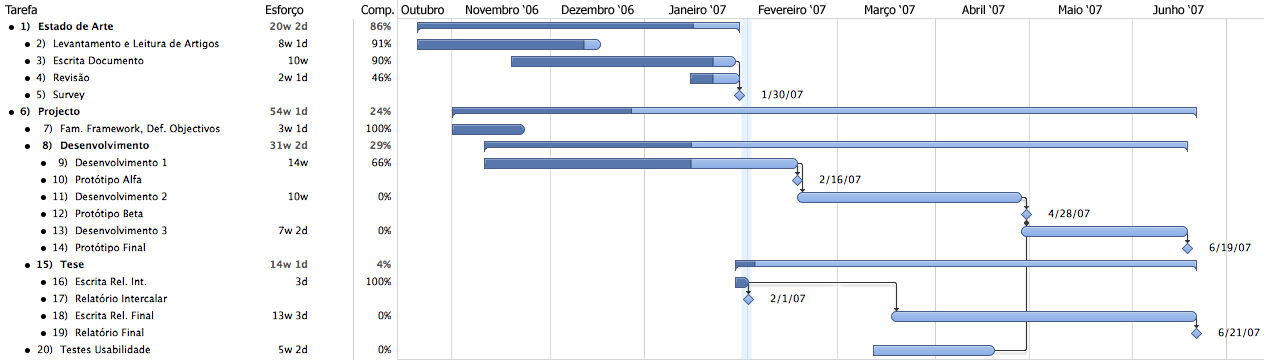
\includegraphics[height=7cm]{gfx/gantt.png}
%	\end{figure}
\end{sideways}
\end{multicols}